\chapter{Implementing an OSGi Bundle Introspection Tool}
This chapter describes how Intrabundle was implemented and architecture overview is presented. Objects and classes that composes it will be detailed. First section gives a general overview of Intrabundle's components, second section explains how OSGi bundles and projects are identified by the tool, next section shows how useful information is being collected and how this information is gathered by reports. Last section gives an overview of how Intrabundle's quality is being maintained.   

\section{Implementation Overview}

Intrabundle is composed by 3 Forge plugins, see section \ref{sec:forge:plugin} for details about Forge plugins. The first is \emph{BundlePlugin} which extracts OSGi bundle information, second is \emph{OSGiPlugin} that has a vision of all bundles composed by the project. Third is \emph{OSGiScan} a plugin responsible for scanning OSGi bundles recursively in file system. 


Intrabundle also provides 2 facets, see section \ref{sec:forge:facet} for details about Forge facets. \emph{BundleFacet} and \emph{OSGiFacet}, both restricts commands provided by BundlePlugin and OSGiPlugin in the context of OSGi bundle and project respectively. BundleFacet is active when user enter on a directory that is an OSGiBundle and OSGiFacet is active when user enters on a directory that contains at least one OSGiBundle. When BundleFacet is active then OSGiFacet is disabled meaning that only BundlePlugin commands will be active. 

Another important component in Intrabundle architecture is the Project Locator, see section \ref{sec:forge:locator} for details about Forge locators. Intrabundle provides 2 locators. The first is \emph{BundleLocator} that creates a Forge project object named \emph{OSGiModule} representing and gathering data related to OSGi bundle. BundleLocator is activated when user is at an OSGi bundle directory. The second is \emph{OSGiProjectLocator} which creates a Forge project object named \emph{OSGiProject} representing an OSGi project which is a collection of bundles. OSGiProject locator is activated when user is in a directory that has at least one child directory that is an OSGiBundle.          

Another component in the architecture is \emph{MetricsCalculator} that calculates bundle and OSGi project quality based on data contained on OSGiProject and OSGiModule objects. To calculate projects qualities Intrabundle creates the \emph{Metric} and \emph{MetricPoints} objects. MetricPoints has a list of Metrics and the quality is calculated in MetricPoints object based on all metrics it has. The final quality is represented by a Java object called \emph{MetricScore} which holds the \emph{quality label} presented in \ref{sec:quality label}.     
Figure \ref{intrabundle-arch} gives an overview of Intrabundle architecture:

\newpage

\begin{figure}[h]
\caption{Intrabundle architecture}
\label{intrabundle-arch}
\centering
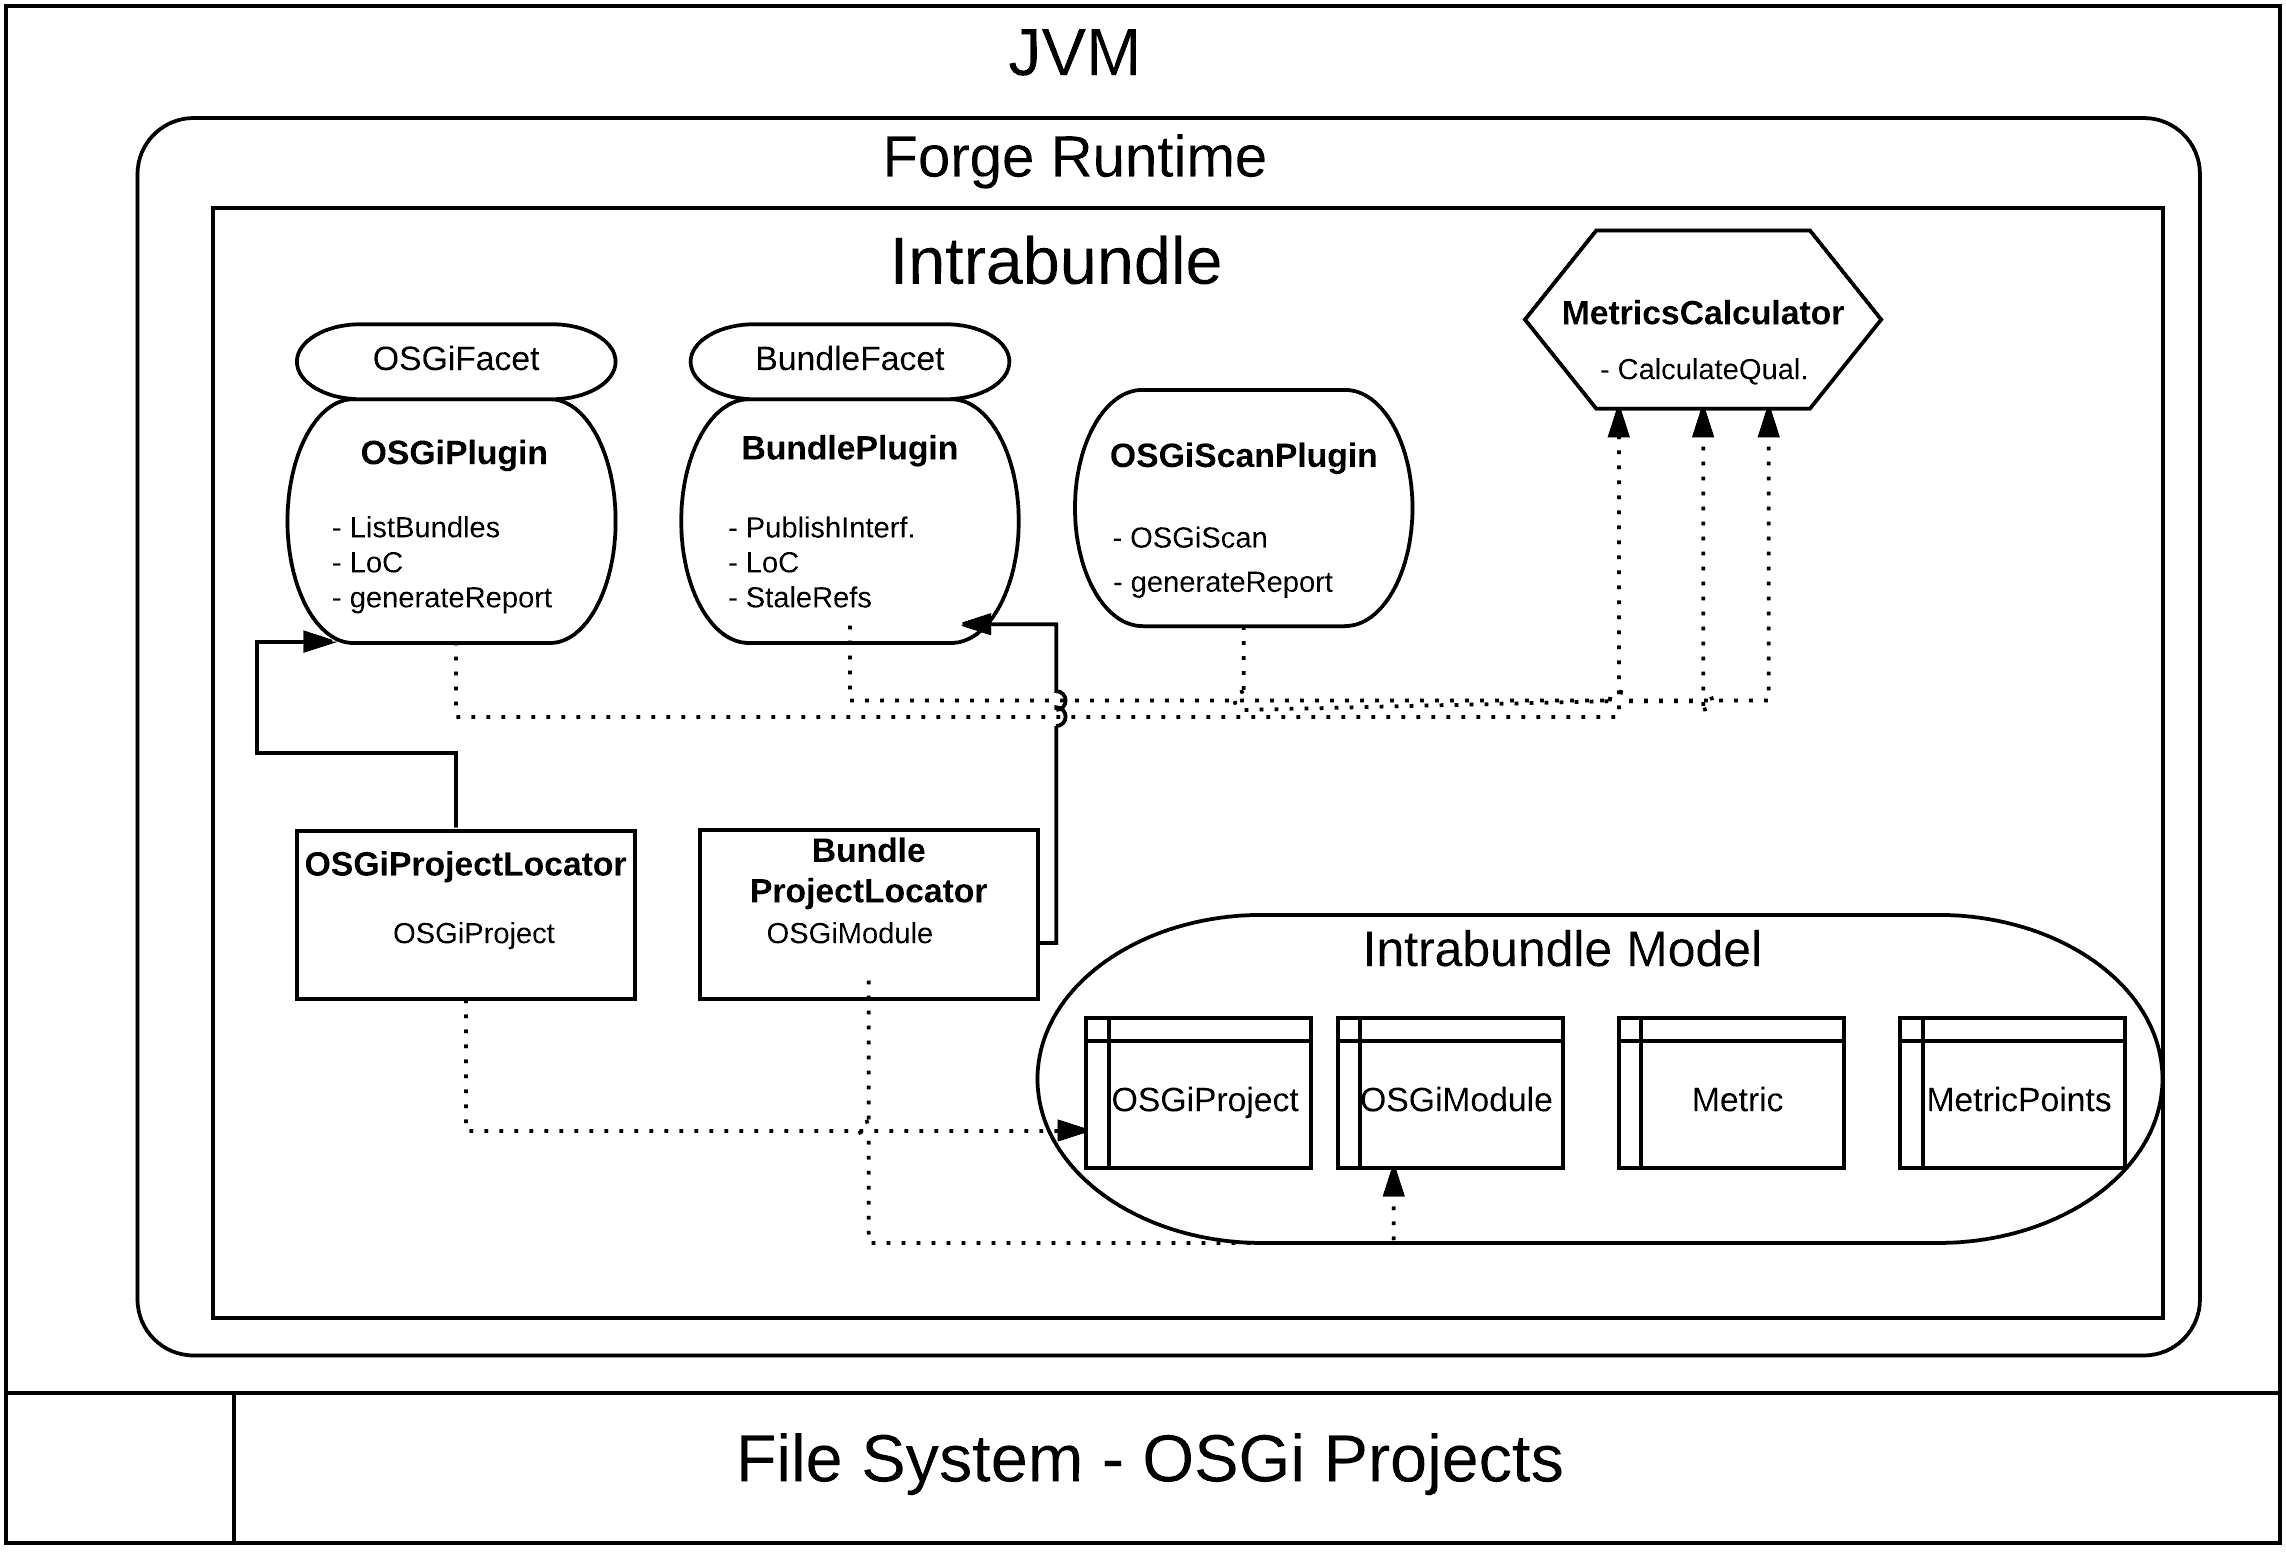
\includegraphics[scale=0.77]{intrabundle-arch}
\end{figure}  
\FloatBarrier


\section{Bundle and Project Identification}

Intrabundle implements its \emph{facets} and \emph{locators} to identify OSGi bundles and OSGi projects. To do that the tool searches for OSGi meta data in \emph{MANIFEST} file\footnote{The manifest is a special file that can contain information about the files packaged in a JAR file. By tailoring this "meta" information that the manifest contains, you enable the JAR file to serve a variety of purposes.}. So identifying bundles is as simple as locating the Manifest and verifies if it's content has OSGi information. The main problem is that the manifest location can vary depending on the project format. Table \ref{osgi-project-type} lists the types of OSGi projects and the location of Manifest file:     

\begin{table}[h]
\caption{Supported types of OSGi projects}
\label{osgi-project-type}
\begin{center}
    \begin{tabular}{  p{4cm} | p{6cm} }
    \Xhline{2\arrayrulewidth}
    Type & Manifest location \\  \hline
    Maven projects & /src/main/resource/META-INF.\\ \hline
    Maven using BND tools & pom.xml\footnote{It's a xml configuration file responsible for project build life cycle and dependencies} with maven-bundle-plugin.\\ \hline
    Standard Eclipse Java projects & /META-INF\\ \hline
    Standard BND Tools & bnd.bnd file in any subfolder.\\ \hline
    Package based bundles & each package has a manifest.\\  
   \Xhline{2\arrayrulewidth}

    \end{tabular}
\end{center}
\end{table}
\FloatBarrier


\section{Retrieving bundle information}
Section \ref{sec:collecting-data} described which information the tool extracts. Now its presented how that is done.


\textbf{LoC} is a classical software metric that was adapted in this work to OSGi Bundles and its calculation is straight forward. The tool just sum the bundle .java files lines of code. It is important to note that comments are excluded from this calculation. 
\textbf{IPojo}, \textbf{Blueprint} and \textbf{Declarative Services} are extracted by looking for specific file configurations(xml files) or annotations that each technology uses.
\textbf{Stale Services references} are detected via approximation, Intrabundle counts the number of services \emph{gets} and \emph{ungets}\footnote{Operations that consume and release a service reference respectively} for each class a bundle has. If the number of gets and ungets are equal then the class have no stale references, otherwise it is considered as having stale references.
\textbf{Bundle dependencies} are calculated by looking at OSGi Manifest file in exported and imported packages. If bundle A \emph{imports} package \emph{x.y.z} and bundle B \emph{exports} package \emph{x.y.z} we say that bundle A depends on bundle B. 
\textbf{Required bundles} just counts the number of required bundles declared in manifest.
\textbf{Publishes interfaces} looks at bundle exported packages, if all exported packages contains only interfaces we say that bundle only publishes interfaces.
\textbf{Declares permission} verifies if bundle implements security by contract searching for \emph{permission.perm} file inide OSGI-INF bundle directory.

Each information retrieved by Intrabundle is usually mapped to a Forge command, see Listing \ref{forge_command_example} which is the command that prints bundle exported packages, an information used to calculate bundle dependency and publish interfaces metric, to the Forge console:
\pagebreak


\begin{lstlisting}[language=java,label=forge_command_example,caption=Exported packages command]
 @Command(value = "exportedPackages",help = "list bundle exportedpackages")
 public void exportedPackages(PipeOut out){
      if(bundle.getExportedPackages().isEmpty()){
            out.println(messageProvider.getMessage("module.noExportedPackages"));
        }
      else{
          for (String s : bundle.getExportedPackages()) {
               out.println(s);
           }
       }
    }
\end{lstlisting}
\FloatBarrier

All the logic is inside \textbf{bundle} variable which is of type \emph{OSGiModule}\footnote{The bundle variable is created by Bundle Locator, a Forge locator, when user navigates to a directory which is an OSGi bundle, as explained in section \ref{sec:forge:locator}.}, that is an immutable object\footnote{Is an object whose state cannot be modified after it is created. A good practice and core principle in domain driven design \citep{Evans 2003}}, in method \emph{getExportedPackages}. All information described in table \ref{extracted-data}, except bundle dependency, is calculated inside OSGiModule object. Bundle dependency is Calculated by OSGiProject because it has all modules and can calculate its dependencies. Above is OSGiModule Java interface describing all operations it provides:\newpage

\begin{lstlisting}[language=java,label=Intrabundle OSGiModule,caption=Intrabundle OSGiModule interface]
public interface OSGiModule extends Serializable, Comparable<OSGiModule>{

    /**
     *
     * @return total .java files(under src or src/main/java) lines of code
     */
    Long getLinesOfCode();


    /**
     * @return <code>true</code> if bundle uses declarative services specification
     * <code>false</code> if it doesnt
     */
    Boolean getUsesDeclarativeServices();

    /**
     * @return <code>true</code> if bundle uses Blueprint specification
     * <code>false</code> if it doesnt
     */
    Boolean getUsesBlueprint();

    /**
     *
     * @return object representing bundle MANIFEST.MF  or .bnd or pom.xml with maven-bundle-plugin
     */
    ManifestMetadata getManifestMetadata();

    /**
     *
     * @return bundle activator java file
     */
    FileResource<?> getActivator();

    /**
     *
     * @return bundle imported packages
     */
    List<String> getImportedPackages();

    /**
     *
     * @return bundle exported packages
     */
    List<String> getExportedPackages();

    /**
     *
     * @return bundle required bundles
     */
    List<String> getRequiredBundles();

    /**
     * @return <code>true</code> if bundle exported packages contains only interfaces
     * <code>false</code> if it has one or more classes
     */
    Boolean getPublishesInterfaces();

    /**
     *
     * @return <code>true</code> if bundle declares permissions
     * <code>false</code> otherwise
     */
    Boolean getDeclaresPermissions();

    /**
     *
     * @return .java files possibly containing OSGi service stale references
     */
    List<Resource<?>> getStaleReferences();
}
\end{lstlisting}
\FloatBarrier


\section{Intrabundle Reports}
\label{sec:intrabundle-reports}
The tool generates two reports based on information it collects from bundles so the it can be analyzed carefully in one place. The reports can be generated in various formats (txt, pdf, html, csv and excel). Figure \ref{intrabundle-report1} shows an example report:  

\begin{figure}[h]
\caption{Intrabundle general report}
\label{intrabundle-report1}
\centering
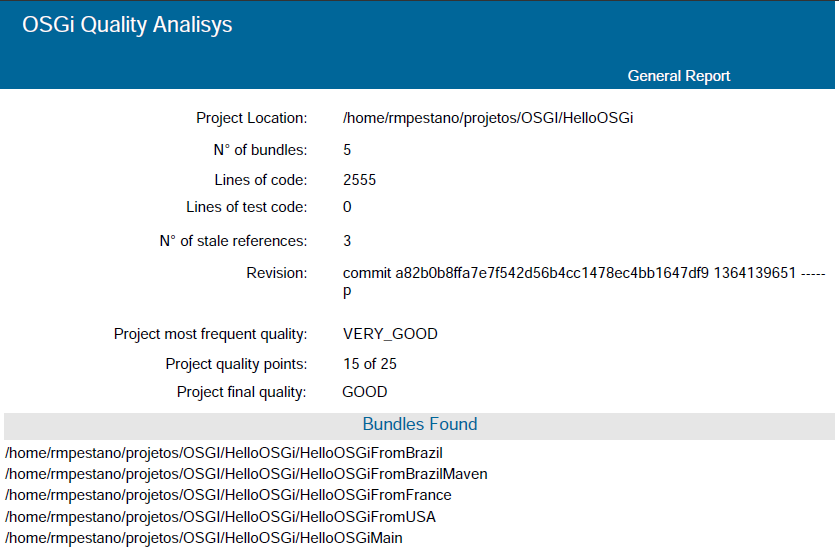
\includegraphics[scale=0.5]{intrabundle-report}
\end{figure}  
\FloatBarrier

The first section of the report gives an overall idea of the project, second part lists information of each bundle, see Figure \ref{intrabundle-report2} 

\begin{figure}[h]
\caption{Intrabundle general report - detailed section }
\label{intrabundle-report2}
\centering
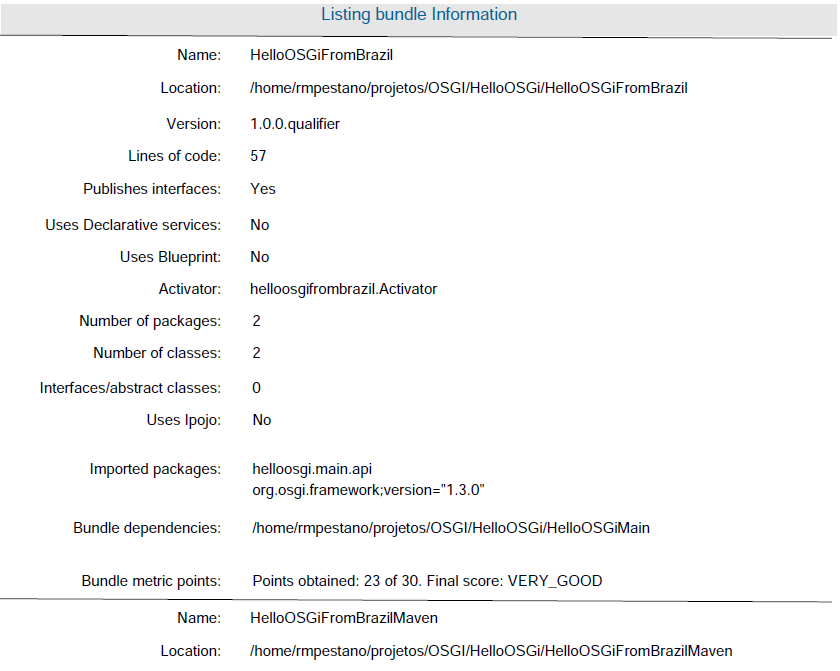
\includegraphics[scale=0.5]{intrabundle-report2}
\end{figure}  
\FloatBarrier

Another report Intrabundle generates is a metric report that details the punctuation of each metric, see Figure \ref{intrabundle-metrics-report}:  

\begin{figure}[h]
\caption{Intrabundle metrics report}
\label{intrabundle-metrics-report}
\centering
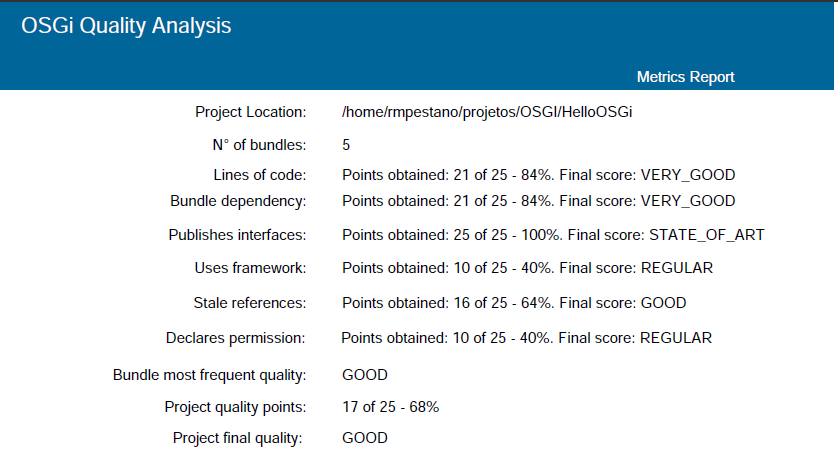
\includegraphics[scale=0.5]{intrabundle-metrics-report}
\end{figure}  
\FloatBarrier

As in general report, in metrics report the first section of the report gives an overall idea of the project, second part lists information of each bundles, see Figure \ref{intrabundle-metrics-report2} 

\begin{figure}[h]
\caption{Intrabundle metrics report - detailed section}
\label{intrabundle-metrics-report2}
\centering
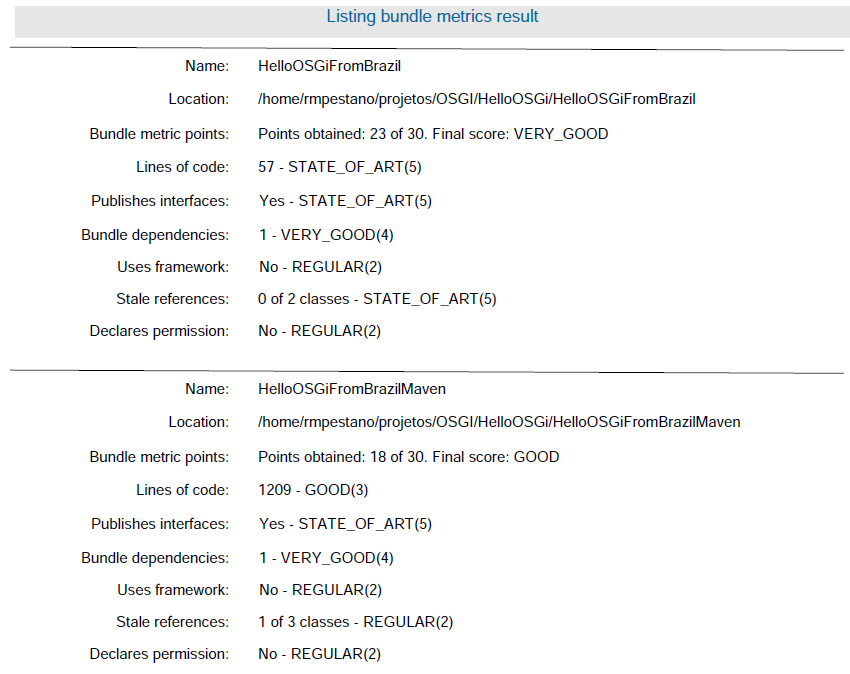
\includegraphics[scale=0.5]{intrabundle-metrics-report2}
\end{figure}  
\FloatBarrier

All reports generated by Intrabundle can be found online \citep{intrabundle reports 2014}.

\section{Intrabundle Quality}
In this section we will see how Intrabundle's quality is managed and how some concepts of \textit{section \ref{sec:quality}} were applied to the project. As the project is not OSGi based we can't apply Intrabundle's metrics on itself so we used classical approaches to assure the quality of the project.

\subsection{Internal quality}
Intrabundle internal quality is managed by PMD and JaCoCo. PMD is an static analysis tool and JaCoCo a dynamic analysis one. Both were presented in section \ref{ch2:qatools} with the objective to guarantee non functional requirements.

\subsubsection{Example}
 PMD was already illustrated at Chapter 2 as an example of static analysis tool. JaCoCo is used to calculate code coverage to track files and methods that automated tests are covering. Figure \ref{intrabundle-code-cover} shows JaCoCo code coverage report for Intrabundle:

\begin{figure}[h]
\caption{Intrabundle code coverage}
\label{intrabundle-code-cover}
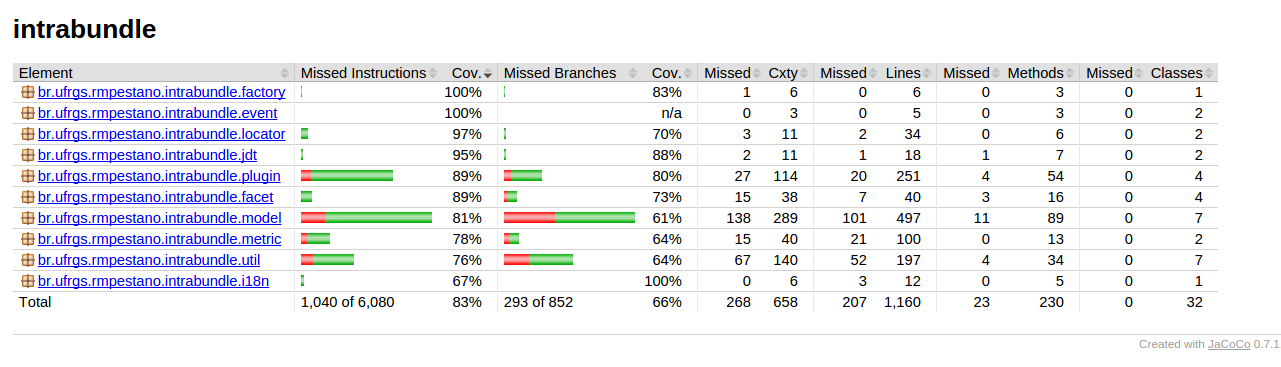
\includegraphics[scale=0.5]{intrabundle-code-coverage}
\end{figure}

\FloatBarrier
\newpage
\subsection{External quality}
Intrabunde external quality is assured by automated whitebox tests so we can verify if Intrabundle is working as expected, if it meets its functional requirements.

\subsubsection{Example}
As of November 2014 Intrabundle performs 65 \textbf{integration tests} which can be defined as automated tests aimed to detect any inconsistencies between the software units that are integrated together. In this kind of automated tests the system must be running and in case of Intrabundle we also need the Forge runtime up during tests. That is done by Arquillian \citep{dan 2011}, an integration testing platform. The tests are also executed online on each commit\footnote{A command that pushes software changes to version control} by \href{https://travis-ci.org/rmpestano/intrabundle}{Travisci}\footnote{An online continuous integration server}, a technique called \emph{continuous integration}. Figure \ref{intrabundle-integ-tests} shows the result of integration tests execution:

\begin{figure}[h]
\caption{Intrabundle integration tests}
\label{intrabundle-integ-tests}
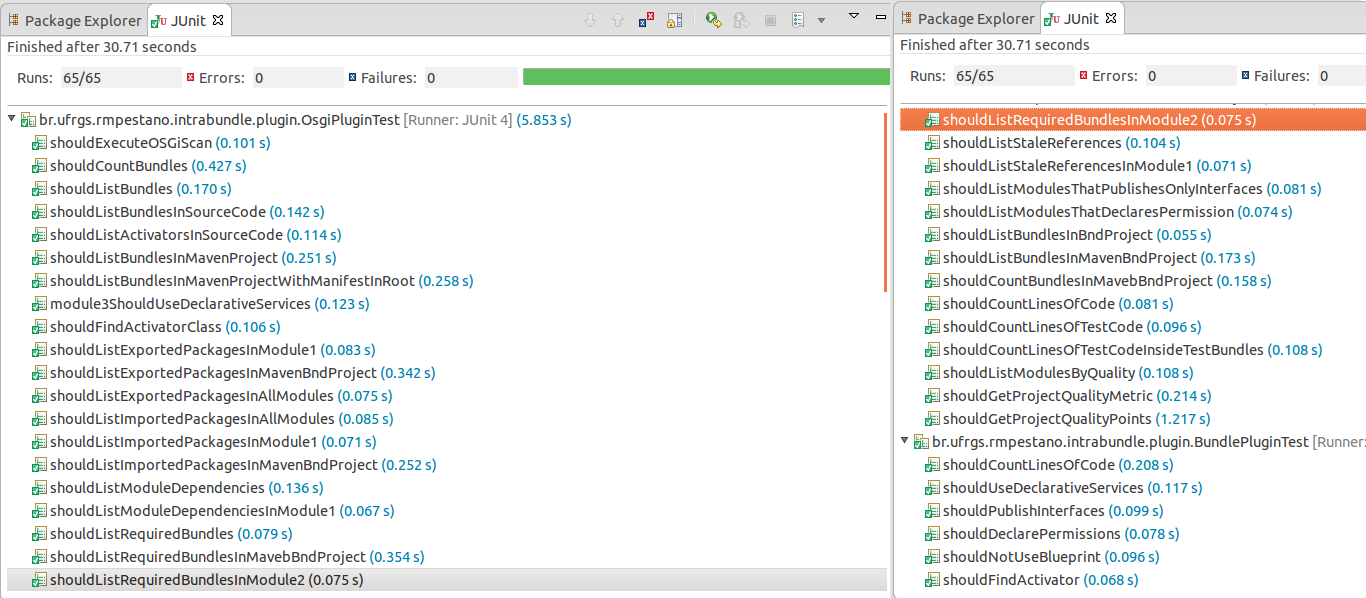
\includegraphics[scale=0.45]{intrabundle-external-quality}
\centering
\end{figure}

\FloatBarrier

\section{Validation}
In order to validate our implementation and if proposed metrics make sense we will generate Intrabundle reports on top 10 real OSGi projects. These reports will be analyzed and we will try to infer useful information and tendencies from them. The reports must gather information that make it possible to compare and confront data in the most variable scenarios.